\chapter{Feedforward-Feedback Steering Controller} 
\label{chapter2}

 A central control task in the operation of an autonomous vehicle is the ability
to maneuver along a desired path, typically generated by a high-level path planner. As a result, a large research effort has been 
devoted to the subject of active steering control for autonomous or semi-autonomous vehicles. Steering systems based on feedback-feedforward (FB-FFW)
control architectures have been a major focus of research. Early
 work by Shladover et al. \cite{shladover} described a FB-FFW controller where the feedforward
steering angle was determined from path curvature and longitudinal force inputs, and the feedback gains were 
selected from a frequency shaped linear quadratic regulator (FSLQR) designed to
 minimize path tracking error while maintaining good ride quality at different frequencies. Nagai et al. \cite{nagai} also used LQR to design two feedback steering controllers for autonomous path following, with one controller using steer angle as the control input
and the other using steering torque. 

Another simple but effective approach to feedback-feedforward steering control is to design a controller with the objective of
making the lateral tracking error zero at a certain ``lookahead" point in front of the vehicle. Minimization of a lookahead
objective was studied by Hingwe and Tomizuka \cite{hingwe}.
A crucial result was the finding that internal yaw dynamics can be damped at all longitudinal velocities by making the
lookahead point a quadratic function of the vehicle velocity. Rossetter \cite{rosseter} also studied lookahead feedback systems extensively,
and derived a similar controller by minimizing a quadratic potential function of the projected lookahead error. 

While initial work was focused at driving well below the limits of tire friction, several
authors obtained respectable results by applying similar methods for more aggresive maneuvers. M{\"u}ller-Be{\ss}ler 
applied a linear plant inversion method to determine feedforward commands for a Volkswagen Golf attempting an aggressive double lane change
maneuver \cite{bessyboy}. Additionally, Thommyppillai et al. \cite{tommyboy} and Sharp et al. \cite{sharpysharp} used a linear preview controller
to simulate path following of a virtual racecar driver. The tendency for linear controller designs to work reasonably well at the limits
 of handling was partially explained by Talvala et al. \cite{talvala}, who were able to find a Lyapunov function demonstrating stability of lookahead steering feedback 
 even in the presence of significant front and rear tire saturation. 

More recent work has focused on improving control performance by accounting for the nonlinear effect of tire saturation at the handling limits. 
Kritiyikarana and Gerdes \cite{mickcop} proposed a force-based FB-FFW controller with the feedforward steering force
 determined by eliminating the error dynamics about the vehicle's center of percussion. The effect of tire saturation was accounted
 for by inverting a nonlinear vehicle dynamics model to convert the desired steering force to a steer angle input. 
Most recently, the emerging trend of model-predictive control has resulted in steering controllers that 
attempt to track a path at the handling limits while also avoiding obstacles. In 2013, Carvalho et al. \cite{carvalho13} demonstrated a model predictive controller (MPC) 
capable of steering an experimental passenger sedan around obstacles at high speeds on an icy road. The controller was based 
on a nonlinear Ackermann model that was iteratively linearized. A similar affine linearization MPC technique was employed by Funke \cite{joethesis} to demonstrate
a student-built vehicle tracking an oval path at accelerations of 8.5 $\mathrm{m/s^2}$ while avoiding rapidly emerging obstacles.  

In summary, there are a wide variety of published steering controllers with varying levels of complexity. However, there is no
 single experimentally validated controller that displays a well-understood combination of robust stability margins
 and low path tracking error at the limits of handling.  The stability properties of lookahead steering below and at the handling
 limits are demonstrated by Rossetter \cite{rosseter} and Talvala \cite{talvthesis}, but with but no discussion of how
 path tracking behavior changes as the vehicle approaches the limits of handling.
Work presented by Kritayakirana and Gerdes \cite{mickcop} was validated
experimentally and has desirable stability properties, but will exhibit non-zero
 path tracking errors below the handling limits with perfect knowledge of the vehicle dynamics.  
range of vehicle accelerations. Experimentally validated results using model-predictive control \cite{carvalho13}\cite{joethesis} demonstrate the ability to balance competing
objectives of vehicle path tracking and stability when the front or rear tires are saturated, but 
consist of complex optimization problems that make fundamental issues such as stability and closed-loop tracking performance difficult to analyze mathematically or
understand qualitatively. 

This chapter therefore presents the design of a feedback-feedforward steering controller that maintains vehicle stability at the handling limits
along with strong path tracking performance where physically possible. 
 A baseline controller with lookahead steering feedback and feedforward based on vehicle kinematics and steady-state tire forces
 is presented in \S \ref{sec:controllerC2}. By focusing on handling characteristics and vehicle kinematics, the feedforward component is able to
remain consistent with the lookahead objective of the steering feedback.  
Section \ref{sec:predSS} uses steady-state simulation results to show this baseline controller will exhibit 
significant path tracking errors at both low and high vehicle lateral accelerations. 
 In \S \ref{sec:betafb}, we consider a modified steering feedback that aims to keep the vehicle sideslip tangent to the desired path. This approach results
 in a closed-loop steering
response with zero steady-state lateral path deviation, but at the cost of poor stability margins. A better
 design approach, presented in \S \ref{sec:goodFFW}, 
is to incorporate the desired sideslip behavior
as a feedforward input, which significantly improves path tracking while maintaining robust stability margins. 
Section \ref{sec:expresults}  provides experimental path tracking data collected
on an Audi TTS test vehicle at Thunderhill Raceway in Willows, California, with
 combined lateral and longitudinal accelerations up to 9.5 $\mathrm{m/s^2}$. 

 \section{Path Description}
 
The objective of the steering controller presented in this chapter is to follow a path generated by a separate high 
level controller. While there are several ways to mathematically represent the coordinates of a desired path, the controller
design will assume the desired trajectory is defined as a series of curvilinear $\left(s, \kappa(s)\right)$ coordinates, where 
$s$ is the distance along the path and $\kappa(s)$ is the instantaneous path curvature. This coordinate system is chosen
because the curvature of a path is very intuitive to map into a desired lateral vehicle force, and ultimately a desired
vehicle steering input. The chosen path description is illustrated
for a simple path in Figure \ref{fig:pathFig}. 

 \begin{figure}[h]
\centering
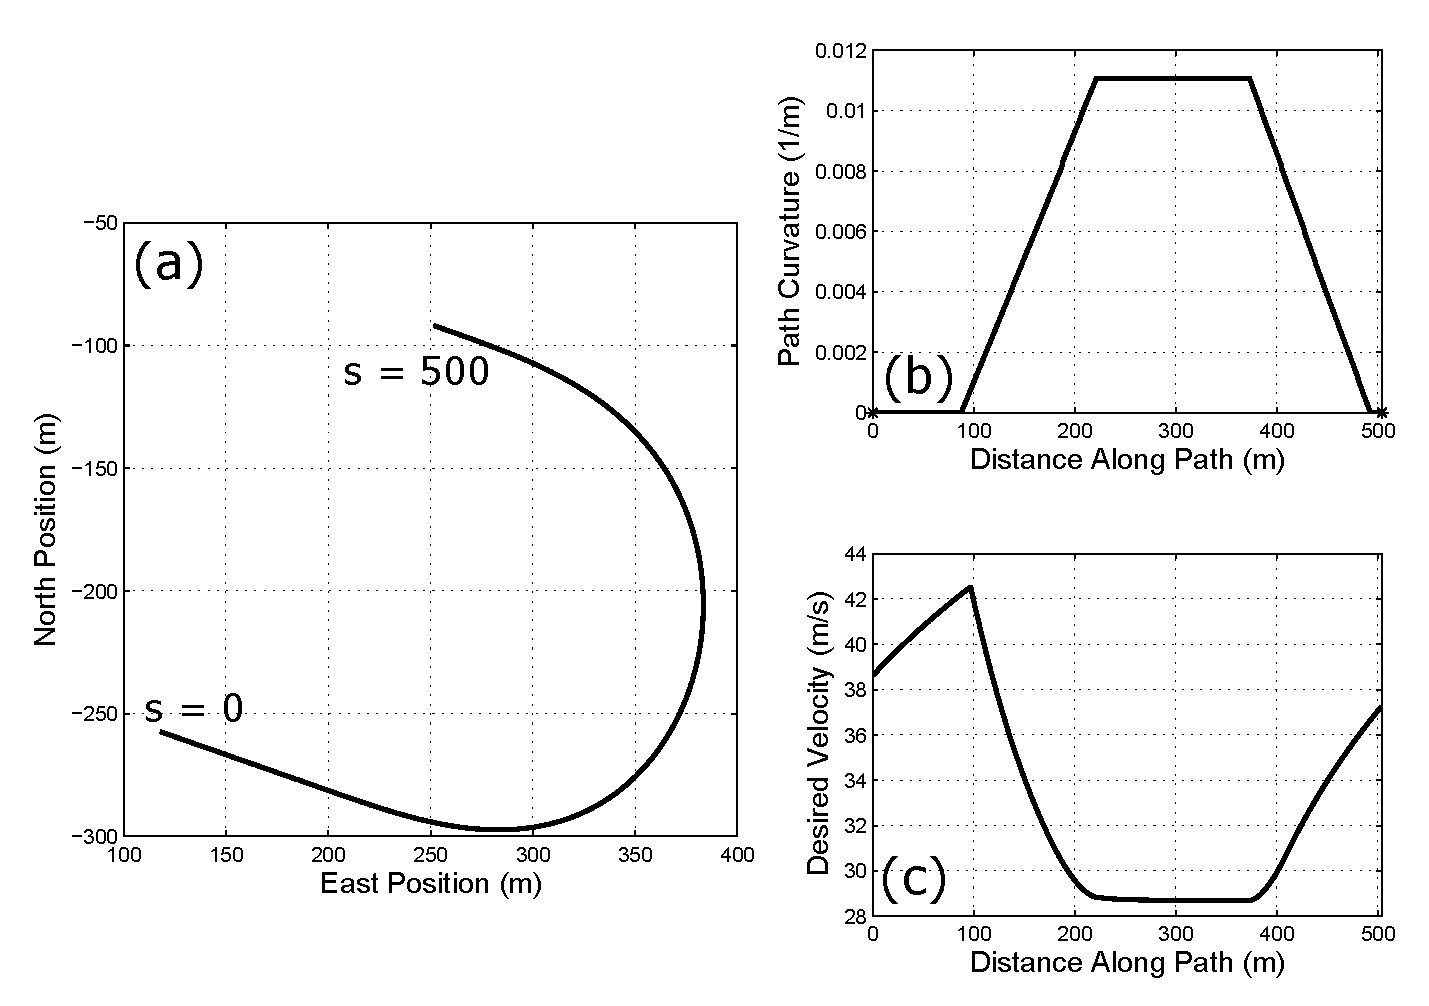
\includegraphics[width=\fullwidth]{pathOverview.eps}
\caption[Path coordinate system]{(a) A 500 meter path plotted in Cartesian coordinates. (b) Curvature profile $\kappa(s)$ as function of 
path length $s$ for associated path. (c) Example velocity profile $(s, U_x^\mathrm{des}(s))$ for path.}
\label{fig:pathFig}
\end{figure}

\newpage
Additionally, given the speed dependence of an automobile's steering dynamics, 
the steering controller also requires knowledge of the desired speed profile (Figure \ref{fig:pathFig}(c)), which must also come from
the high level trajectory planner. The speed profile can be represented as a series of $(s, U_x^\mathrm{des}(s))$ coordinates,
where $U_x^\mathrm{des}(s)$ is the desired speed at a given distance along the path. 
 


%For the experimental data validation presented in this chapter, the desired path curvature is provided to the
% controller via the path planning algorithm  from Theodosis \cite{theodosis}. This algorithm outputs planned trajectories
% where $\kappa$ is a piecewise-linear function of $s$. Additionally, the velocity profile is obtained
% from a longitudinal controller developed by Kritayakirana that keeps the combined vehicle acceleration magnitude at a specified
% value \cite{mickcop}. 
 
\section{Controller Architecture}
\label{sec:controllerC2}

A block diagram of a typical feedback-feedforward structure for steering control is shown in Fig.~\ref{fig:controllerBD}. Inputs to the feedforward
steering angle $\delta_\mathrm{FFW}$ are the current path curvature $\kappa$ and forward velocity $U_x$. Inputs to the feedback steering angle $\delta_\mathrm{FB}$ are lateral path deviation
$e$ and path heading error $\Delta\Psi$ (Fig.~\ref{fig:bikeModel}). The total steering command $\delta$ is the sum of the feedback and feedforward inputs.

% % % % % % % figure, blockdiagram % % % % % % %
\begin{figure}[h]
\centering
\includegraphics[width=\fullwidth]{FB_FFW.png}
\caption{Block diagram of feedback-feedforward steering controller.}
\label{fig:controllerBD}
\end{figure}
% % % % % % % end figure % % % % % % %

 

\subsection{Feedforward Steering Design}
\label{sec:baselineFFW}

The objective of the steering feedforward is to provide an estimate of the steer angle required to traverse a path with a known path curvature and velocity profile.
This minimizes the level of compensation required by the steering feedback, reducing tracking errors and allowing for less overall control effort. 
To simplify the controller structure, the feedforward steering angle should depend only on the desired trajectory and be independent of the actual vehicle states.

The proposed structure of the steering feedforward begins with the assumption that vehicle dynamics are given by the planar ``bicycle" model,
 with relevant vehicle states and dimensions shown in Fig.~\ref{fig:bikeModel} and described in Table \ref{tb:bikeModelDefns}. The planar bicycle model makes the
key assumption that the left and right tires act to produce a single combined lateral force, resulting
in just two lateral forces $F_\mathrm{yf}$ and $F_\mathrm{yr}$ acting at the front  and rear. Actuation of steer angle $\delta$
at the front tire results in generation of the lateral tire forces through the tire slip angles $\alpha_\mathrm{f}$ and $\alpha_\mathrm{r}$. 
The two resulting states that evolve are vehicle yaw rate $r$, which describes the vehicle angular rotation,
 and sideslip $\beta$, which is the ratio of lateral velocity $U_y$ to longitudinal velocity $U_x$.  
 
  \begin{table}[h]
\begin{center}
\caption{Bicyle Model Definitions}\label{tb:bikeModelDefns}
\begin{tabular}{lcc}
Parameter & Symbol & Units \\\hline
Front axle to CG & $a$ & m\\
Rear axle to CG & $b$  & m\\
Front Lateral Force & $F_\mathrm{yf}$ & N\\
Front Tire Slip     & $\alpha_\mathrm{f}$ & rad \\
Rear Lateral Force & $F_\mathrm{yr}$ & N\\
Rear Tire Slip     & $\alpha_\mathrm{r}$ & rad \\
Steer Angle Input  & $\delta$           & rad \\
Yaw Rate   & $r$ & rad/s \\
Sideslip   & $\beta$ & rad \\
Lateral Path Deviation & $e$ & m \\
Heading Deviation & $\Delta\Psi$ & rad \\
Longitudinal Velocity & $U_x$ & m/s \\
Lateral Velocity & $U_y$ & m/s \\\hline
\end{tabular}
\end{center}
\end{table}
 
 In addition to the two vehicle states $\beta$ and $r$, two additional states are required to describe the vehicle's
 position relative to the desired path. These are also shown in Fig.~\ref{fig:bikeModel}. The lateral path deviation,
 or lateral error, $e$, is the distance from the vehicle center of gravity to the closest point on the desired path. 
 The vehicle heading error $\Delta\Psi$ is defined as the angle between the vehicle's centerline and the tangent line
 drawn on the desired path at the closest point. 
\begin{figure}[h]
\centering
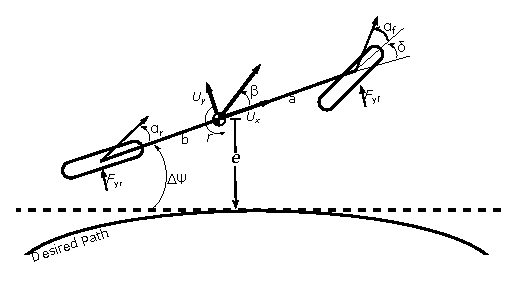
\includegraphics[width=.75\fullwidth]{BikeModelSchematic.eps}
\caption[Schematic of planar bicycle model]{Schematic of planar bicycle model.}
\label{fig:bikeModel}
\end{figure}
Note that the longitudinal dynamics of the vehicle are not explicitly
 modeled in this formulation. Instead of keeping the longitudinal velocity $U_x$ as a vehicle state, the longitudinal
 velocity is treated as a time-varying parameter. 

The problem of determining suitable feedforward lateral tire forces for autonomous path following was studied by Krisada and Gerdes \cite{mickcop}. The (linearized) equations of 
motion for the states shown in Fig.~\ref{fig:bikeModel} are given by:

\begin{subequations}
\label{eq:bm}
\begin{align}
	\dot{\beta} &= \frac{F_\mathrm{yf}+F_\mathrm{yr}}{mU_x} - r \label{eq:bm1}\\
	\dot{r} &= \frac{aF_\mathrm{yf} - bF_\mathrm{yr}}{I_z} \label{eq:bmc2} \\
	\dot{e} &= U_x (\beta + \Delta\Psi) \label{eq:bm3} \\
	\Delta\dot{\Psi} &= r - \dot{s}\kappa \label{eq:bm4} 
\end{align}
\end{subequations}
where $m$ and $I_z$ are the vehicle mass and out-of-plane rotational inertia, and $s$ is the distance along the desired path. Taking time derivatives of $\dot{e}$ and $\Delta\dot{\Psi}$ and substituting from (\ref{eq:bm1}) and (\ref{eq:bmc2}) yields:

\begin{subequations}
\label{eqn:doubleds}
\begin{align}
	\ddot{e} &= \frac{F_\mathrm{yf}+F_\mathrm{yr}}{m} - U_x\kappa\dot{s} \\
	\Delta\ddot{\Psi} &= \frac{aF_\mathrm{yf} - bF_\mathrm{yr}}{I_z} -\kappa\ddot{s} - \dot{\kappa}\dot{s}
\end{align}
\end{subequations}
In general, the values chosen for the feedforward front and rear tire forces $F_\mathrm{yf}$ and $F_\mathrm{yr}$ should
bring $\ddot{e}$ and $\Delta\ddot{\Psi}$ to zero. However, for a typical front-steer vehicle, 
direct control is only available for the front steering force $F_\mathrm{yf}$ via command of the steering input $\delta$. The rear tire
force depends indirectly on the steering angle via the build-up of rear tire slip $\alpha_\mathrm{r}$. It is therefore
not possible to simultaneously eliminate both the lateral tracking error and heading angle error. 

An alternative is to consider eliminating a weighted combination of the two error states by eliminating the lateral tracking 
error $e_p$ at a specified point $x_p$ in front of the vehicle, as shown in Fig.~\ref{fig:projerr}. The error dynamics at this projected point are given by: 

\begin{subequations}
\label{eqn:xp}
\begin{align}
	e_p        &= e + x_p\Delta\Psi \\
	\ddot{e}_p &= \frac{F_\mathrm{yf} + F_\mathrm{yr}}{m} - U_x\kappa\dot{s} + x_p\frac{aF_\mathrm{yf} - bF_\mathrm{yr}}{I_z} - x_p(\kappa\ddot{s} + \dot{\kappa}\dot{s})
\end{align}
\end{subequations}

\begin{figure}[h]
\centering
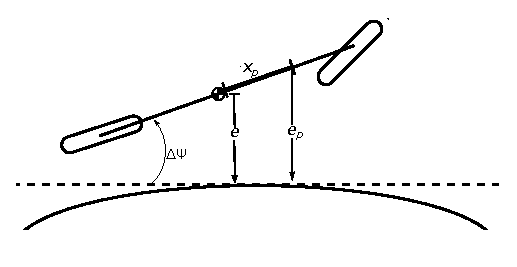
\includegraphics[width=.8\fullwidth]{epfig.eps}
\caption{Projection of lateral error at distance $x_p$ in front of the center of gravity.}
\label{fig:projerr}
\end{figure}

Kritayakirana and Gerdes \cite{mickcop} proposed the center of percussion $x_\mathrm{cop} = \frac{I_z}{bm}$ as a convenient projection point
for the feedforward steering. Substituting $x_p = x_\mathrm{cop}$ and $\ddot{e}_\mathrm{cop} = 0$  yields a simplified equation for the front tire force:

\begin{equation}
\label{eqn:xcop}
 F_\mathrm{yf} = \frac{mb}{L}\left(U_x^2\kappa + x_\mathrm{cop}(\kappa\ddot{s} + \dot{\kappa}\dot{s})\right)
\end{equation}

The benefit of choosing the center of percussion becomes clear in (\ref{eqn:xcop}). The error dynamics at the
center of percussion are independent of the rear tire force, which can be highly transient when the vehicle is cornering near the
limits of handling. This leaves the only control input as $F_\mathrm{yf}$, which can be directly
manipulated by the front wheel steering. 

A feedforward steering approach based on eliminating tracking error at the center of percussion performed well experimentally at lateral accelerations up to
7-8 $\mathrm{m/s^2}$ \cite{mickcop}. However, at higher lateral accelerations, the closed-loop steering response became underdamped, and
the result was significant levels of yaw rate and steering wheel oscillation. This was due to the difficulty of translating a
desired front tire force $F^\mathrm{FFW}_\mathrm{yf}$ into the required steering angle $\delta_\mathrm{FFW}$. 
In general, this relationship is dependent on the vehicle yaw rate $r$ and sideslip $\beta$:

\begin{equation}
\label{eqn:bikeffw}
\delta_\mathrm{FFW} = \frac{U_x\beta + ar}{U_x} - f^{-1}(F^\mathrm{FFW}_\mathrm{yf})
\end{equation}
where $f^{-1}(F_\mathrm{y})$ is an inverse tire model relating tire force to tire slip. This raises the question of 
whether to use actual vehicle states or predicted vehicle states from the bicycle model. Using actual states
results in undesirable coupling between the feedback and feedforward controller and oscillations due to transient vehicle dynamics and 
delays in the steering system, while using predicted states will result in inaccurate tire forces if the vehicle deviates from the desired trajectory.

To eliminate yaw rate oscillation and the dependence on sideslip and yaw rate states,
 we propose simplifying the feedforward tire forces by assuming steady-state cornering conditions. Setting $\dot{s} = U_x$, $\ddot{s} = \dot{\kappa} = 0$
in (\ref{eqn:xcop}) and $\dot{r} = 0$ in (\ref{eq:bm}) yields the following front and rear tire forces:

\begin{subequations}
\label{eqn:ffwforces}
\begin{align}
  F_\mathrm{yf}^\mathrm{FFW} = \frac{mb}{L} U_x^2\kappa\\
   F_\mathrm{yr}^\mathrm{FFW}=\frac{ma}{L} U_x^2\kappa
   \end{align}
\end{subequations}

At steady-state conditions and assuming small angles, the feedforward steering angle of the vehicle relates to the front and 
rear lateral tire slip $\alpha_\mathrm{f}$ and $\alpha_\mathrm{r}$ and path curvature $\kappa$ by vehicle kinematics:

\begin{equation}
\label{eqn:steadyffw}
\delta_{\mathrm{FFW}} = L\kappa - \alpha_\mathrm{f}^\mathrm{FFW}+\alpha_\mathrm{r}^\mathrm{FFW}
\end{equation}
where $\alpha_\mathrm{f}^\mathrm{FFW}$ and $\alpha_\mathrm{r}^\mathrm{FFW}$ are the lumped front and rear feedforward tire slip angles. Notice that
 (\ref{eqn:ffwforces}) and (\ref{eqn:steadyffw}) result in a vehicle feedforward based on a steady-state force balance and vehicle kinematics as opposed
to minimizing error about a point such as the center of percussion (\ref{eqn:xcop}). As a result, there are no compatibility issues
 when combining the feedforward with a lookahead steering feedback. 

The choice of feedforward tire slip angles is related to the tire forces in (\ref{eqn:ffwforces}) via the inverted tire model $f^{-1}(F_\mathrm{y})$. 
To account for saturation of tire force with increasing tire slip magnitude, a single friction coefficient brush Fiala model \cite{Pacejka2012} maps lateral 
tire slip angles into tire force as follows: 
\begin{eqnarray}
\label{eqn:fiala}
	F_\mathrm{y\diamond}&=&\begin{cases} -C_{\diamond}\tan\alpha_\diamond + \frac{C_\diamond^2}{3\mu F_\mathrm{z\diamond}} |\tan\alpha_\diamond| \tan\alpha_\diamond \\ \hspace{10mm}- \frac{C_\diamond^3}{27\mu^2F_\mathrm{z\diamond}^2}\tan^3\alpha_\diamond,
\hspace{8mm}  |\alpha_\diamond| < \arctan{\left(\frac{3\mu F_\mathrm{z\diamond}}{C_\diamond}\right)} \\ \\ -\mu F_\mathrm{z\diamond}\text{sgn} \ \alpha_\diamond, \hspace{36mm} \mathrm{otherwise} \end{cases}
\end{eqnarray}
where the symbol $\diamond \in [\mathrm{f},\mathrm{r}]$ denotes the lumped front or rear tire, $\mu$ is the surface coefficient of friction, and $C_\diamond$ and $F_\mathrm{z\diamond}$ are the corresponding cornering stiffness and normal
load parameters. The cornering stiffnesses and friction coefficient are determined from experimental data taken from a ramp-steer maneuver, as shown in Fig.~\ref{fig:tireCurve}.

\begin{figure}[h]
\centering
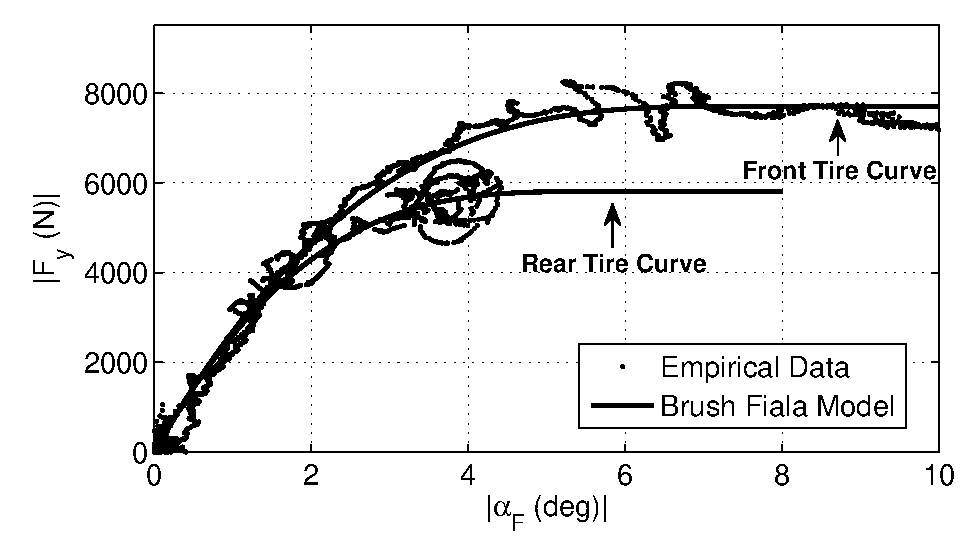
\includegraphics[width=.9\fullwidth]{FrontRearTireCurves.eps}
\caption{Nonlinear tire curves for FFW steering.}
\label{fig:tireCurve}
\end{figure}
\subsection{Feedback Steering Design}
\label{sec:lookahead}

With the feedforward design complete, the remaining step is to design the feedback controller. The goal of the feedback controller is to
minimize a \textit{lookahead} error $e_\mathrm{LA}$, which is the vehicle tracking error projected a distance 
$x_\mathrm{LA}$ in front of the vehicle (Fig.~\ref{fig:lookaheadSchematic}).

\begin{figure}[h]
\centering
\includegraphics[width=.8\fullwidth]{lookaheadSchematic.eps}
\caption{Schematic of planar bicycle model showing projected lookahead error.}
\label{fig:lookaheadSchematic}
\end{figure}

The lookahead error and resulting feedback control law are given by:

\begin{subequations}
\label{eqn:lookahead}
\begin{align}
	e_\mathrm{LA}&=e+x_\mathrm{LA}\Delta\Psi \\
	\delta_\mathrm{FB} &= -k_\mathrm{p}e_\mathrm{LA}
\end{align}
\end{subequations}
with proportional gain $k_\mathrm{p}$. The control law (\ref{eqn:lookahead}) is a natural extension of potential field lanekeeping, as described by Rossetter et al. in \cite{rosseter}, which also provides heuristics for 
selecting $k_\mathrm{p}$ and $x_\mathrm{LA}$. Desirable stability properties of this feedback controller are demonstrated in \cite{talvala}. 

\section{Predicted Steady-State Path Tracking Error}
\label{sec:predSS}

Simulation results provide useful insight about the steady-state path tracking behavior of the baseline feedback-feedforward system. 
Linearized equations of motion for the vehicle and error states can be written in state-space form, with state variable $x$ and control input $\delta$ defined as follows:

\begin{subequations}
\label{eqn:delta}
\begin{align}
		     x &= [e \hspace{2 mm} \Delta\Psi \hspace{2 mm} r \hspace{2 mm} \beta]^T \\
        \delta &=\delta_\mathrm{FB}+\delta_\mathrm{FFW} \\
               &=\left[-k_\mathrm{LK} \hspace{1 mm} -k_\mathrm{LK} x_\mathrm{LA} \hspace{3 mm} 0 \hspace{3 mm} 0\right] x+\left(L+\frac{K_\mathrm{ug} U_x^2}{g}\right) \kappa
\end{align}
\end{subequations}
 where $K_\mathrm{ug}$ is the vehicle understeer gradient, a parameter related to the front/rear weight distribution of the vehicle.
Note that $\delta_\mathrm{FB}$ in (\ref{eqn:delta}b) depends on the state variable, and $\delta_\mathrm{FFW}$ depends on the path curvature. Rewriting  
the vehicle state equations of motion using curvature as the input results in:

\begin{subequations}
\label{eqn:Amatrix}
\begin{align}
    \dot{x} &= Ax + B\kappa  \\
	A  &=  \begin{bmatrix}
   0 & U_x & 0 & U_x \\ 
   0 & 0 & 1 & 0 \\ 
   \frac{-ak_\mathrm{p} C_\mathrm{f}}{I_\mathrm{z}}  & \frac{-ak_\mathrm{p}x_\mathrm{LA}C_\mathrm{f}}{I_\mathrm{z}}  & \frac{-(a^2C_\mathrm{f}+b^2C_\mathrm{r})}{U_xI_\mathrm{z}} & \frac{bC_\mathrm{r} - aC_\mathrm{f}}{I_\mathrm{z}}  \\
   \frac{-k_\mathrm{p}C_\mathrm{f}}{mU_x}  & \frac{-k_\mathrm{p}x_\mathrm{LA}C_\mathrm{f}}{mU_x}  & \frac{bC_\mathrm{r}-aC_\mathrm{f}}{mU_x^2}-1 & \frac{-(C_\mathrm{f} + C_\mathrm{r})}{mU_x}
  \end{bmatrix} \\
	B  &=\left[0 \hspace{2 mm} -U_x \hspace{3 mm} \frac{a C_\mathrm{f} G_\mathrm{FFW}}{I_\mathrm{z}} \hspace{3 mm}  \frac{C_\mathrm{f} G_\mathrm{FFW}}{mU_x}\right]^T
\end{align}
\end{subequations}
where $G_\mathrm{FFW} = (L+\frac{K_\mathrm{ug} U_x^2}{g})$ and $C_\mathrm{f}$ and $C_\mathrm{r}$ are the lumped front and rear cornering stiffnesses. Fig.~\ref{fig:linError} shows results from using the linear model (\ref{eqn:Amatrix}) to compute steady-state path
 tracking errors at the vehicle center of gravity over a range of vehicle speeds, given
 a constant lateral acceleration of $a_y =$ 3 $\mathrm{m/s}^2$. Additionally, steady-state results from the nonlinear feedforward control law 
 (\ref{eqn:steadyffw}) are plotted for the case where $a_y =$ 7 $\mathrm{m/s}^2$. For this high lateral acceleration case, the
 equations of motion (\ref{eq:bm}) and nonlinear Fiala tire model (\ref{eqn:fiala}) are used to predict the steady-state results. In general, steady-state lateral dynamics are reached
within one second for a constant lateral acceleration maneuver. At low lateral accelerations, when the vehicle
 dynamics are dictated by linear equations of motion, the accumulated steady-state tracking error is small ($<$ 0.05 m) at highway speeds. However, 
when steering at the limits of handling, Fig.~\ref{fig:linError} shows that the increased sideslip of the vehicle results
 in higher steady-state tracking error, creating challenges for accurate driving in safety-critical situations. 
 
\begin{figure}[h]
\centering
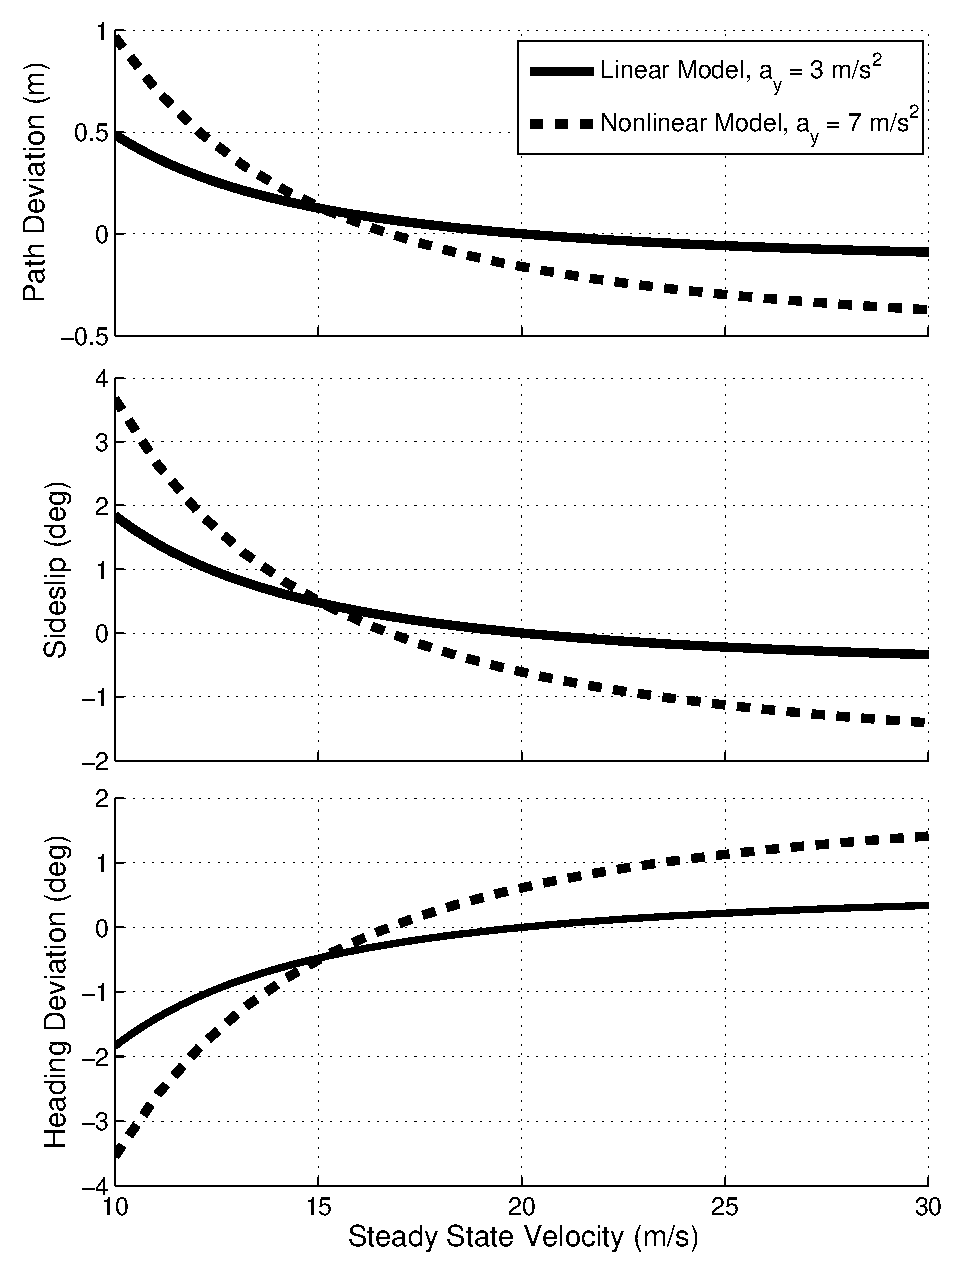
\includegraphics[width=.8\fullwidth]{LinearErrorPlot.eps}
\caption[Steady-state path tracking error $e$, sideslip $\beta$ and heading deviation $\Delta\Psi$ as a function of vehicle speed.]{Steady-state path tracking error $e$, sideslip $\beta$ and heading deviation $\Delta\Psi$ as a function of vehicle speed. Results are plotted for the linear model, with fixed lateral acceleration $a_y = $ 3 $\mathrm{m/s}^2$, and for the
nonlinear model, with fixed lateral acceleration $a_y = $ 7 $\mathrm{m/s}^2$.}
\label{fig:linError}
\end{figure}
 
A qualitative explanation for this steady-state error is shown in Fig.~\ref{fig:SSerror}. Since the steering controller acts to eliminate a weighted
sum of heading error $\Delta\Psi$ and lateral path deviation $e$, the lookahead feedback is successful in
minimizing the desired metric $e_\mathrm{LA}$ at the projected distance $x_\mathrm{LA}$ in front of the vehicle. However, this still allows for steady-state equilibria where
values of $e$ and $\Delta\Psi$ themselves are nonzero.  

\begin{figure}[h]
\centering
\includegraphics[width=.4\fullwidth]{SSerror.png}
\caption{Steady-state cornering where vehicle has lateral error but no lookahead error.}
\label{fig:SSerror}
\end{figure}
 
% % % % % % % end figure % % % % % % %

%=======================================================================
\section{Incorporating Sideslip-Path Tangency into \newline Steering Feedback}
\label{sec:betafb}

An interesting observation from Fig.~\ref{fig:linError} is that the steady-state path deviation
 is zero at a vehicle speed of around $U_x$=20 m/s for the linear model and $U_x$=17 m/s for the nonlinear model. 
 At these speeds, the steady-state vehicle sideslip is predicted to be zero as well, 
and the vehicle heading $\Psi$ naturally becomes tangent to the desired path heading. 

This observation motivates a second form of lookahead feedback where the feedback objective is to maintain the 
vehicle velocity vector $U = \langle U_x \hspace{2mm} U_y \rangle$ tangent to the desired path, as shown in Fig.~\ref{fig:noSSerror}. Since
 the direction of $U$ is given by $\angle U = \Psi+\beta$, the resulting control law is:
 
\begin{subequations}
\label{eqn:vveq}
\begin{align}
        \delta_\mathrm{FB} & = -k_\mathrm{p} \left(e+x_\mathrm{LA} (\angle U-\Psi_\mathrm{r} ) \right) \\
                           & =  -k_\mathrm{p} \left(e+x_\mathrm{LA} (\Psi+\beta-\Psi_\mathrm{r} ) \right) \\
						   & = -k_\mathrm{p} \left(e+x_{LA}(\Delta\Psi+\beta) \right)
\end{align}
\end{subequations}

 \begin{figure}[h]
\centering
\includegraphics[width=.5\fullwidth]{noSSerror.png}
\caption{Zero steady-state lateral deviation requires vehicle velocity vector
to be tangent to path.}
\label{fig:noSSerror}
\end{figure} 
\noindent where $\Psi_\mathrm{r}$ is the heading of the desired vehicle path at a given point. The modified control law can be modeled by reformulating the matrix $A$ in (\ref{eqn:Amatrix}) as:
 
\begin{equation}
\label{eqn:Amatrix2}
A  = 
 \begin{bmatrix}
  0 & U_x & 0 & U_x \\
  0 & 0 & 1 & 0 \\
  \frac{-ak_\mathrm{p} C_\mathrm{f}}{I_\mathrm{z}}  & \frac{-ak_\mathrm{p}x_\mathrm{LA}C_\mathrm{f}}{I_\mathrm{z}}  & \frac{-a^2C_\mathrm{f}-b^2C_\mathrm{r}}{U_xI_\mathrm{z}} & \mathbf{\frac{bC_\mathrm{r} - aC_\mathrm{f}(1-ak_\mathrm{p}x_\mathrm{LA}) }{I_\mathrm{z}}}  \\
  \frac{-k_\mathrm{p}C_\mathrm{f}}{mU_x}  & \frac{-k_\mathrm{p}x_\mathrm{LA}C_\mathrm{f}}{mU_x}  & \frac{-aC_\mathrm{f}-bC_\mathrm{r}}{mU_x^2}-1 & \mathbf{\frac{-(C_\mathrm{f}(1+k_\mathrm{p}x_\mathrm{LA}) + C_\mathrm{r})}{mU_x}}
 \end{bmatrix}
 \end{equation}
  
Note that (\ref{eqn:Amatrix2}) is equal to (\ref{eqn:Amatrix}b) with the exception of the last column, highlighted
in bold. Fig.~\ref{fig:linError2} shows the resulting steady-state behavior, and indicates that lateral error $e$ settles to
zero for all velocities. 

However, the disadvantage of directly adding vehicle sideslip 
into the feedback control is reduced stability margins. Closed-loop eigenvalues of (\ref{eqn:Amatrix}b) and (\ref{eqn:Amatrix2})
are plotted in Fig.~\ref{fig:rLocusPlot} as a function of increasing vehicle speed from 5 m/s to 25 m/s.
\begin{figure}[h]
\centering
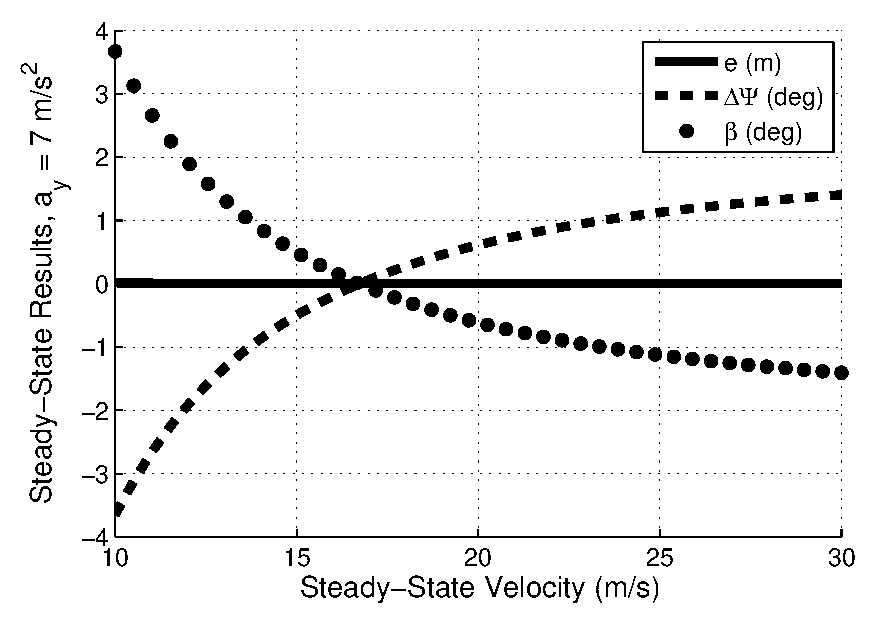
\includegraphics[width=.85\fullwidth]{LinearErrorPlotBeta.eps}
\caption[Steady-state simulation results with sideslip added to feedback control]{Steady-state simulation results with sideslip added to feedback control, using the nonlinear vehicle model with fixed lateral acceleration of 7 $\mathrm{m/s^2}$.}
\label{fig:linError2}
\end{figure} 

The results indicate that the closed-loop steering response
is well-damped ($\zeta =$ 0.9 at a vehicle speed of 25 m/s) with the original lookahead feedback controller. However, when, the steering feedback acts to 
keep the vehicle sideslip tangent to the desired path via (\ref{eqn:vveq}), the closed-loop steering response becomes highly underdamped 
\mbox{($\zeta$= 0.2 at $U_x$ = 25 m/s)}.  

\begin{figure}[h]
\centering
\includegraphics[width=.53\fullwidth]{rLocus.eps}
\caption[Closed-loop pole locations for steering system as vehicle speed is varied from 5 to 25 m/s]{Closed-loop pole locations for steering system as 
vehicle speed is varied from 5 to 25 m/s. Damping ratio $\zeta$ and natural
frequency $\omega_n$ are shown for $U_x$ = 25. Root locus plots are shown for both the lookahead feedback controller (\ref{eqn:Amatrix}) as well as the feedback controller with added
sideslip (\ref{eqn:Amatrix2}). Root locus moves in direction of arrows as vehicle speed is increased.}
\label{fig:rLocusPlot}
\end{figure}
\newpage
Note that the results shown in Fig.~\ref{fig:rLocusPlot} are for a single vehicle and controller parameterization (see Table 1). 
In general, the reduction in stability margin will vary significantly depending on the vehicle understeer gradient and steering controller gains, namely
the lookahead distance. Fig.~\ref{fig:VcrPlot} shows the critical speed $V_\mathrm{cr}$, beyond which the closed-loop 
steering system becomes unstable, for neutral, understeering, and oversteering configurations as a function of $x_\mathrm{LA}$.
For an understeering vehicle, lookahead feedback is always stable as long
as the lookahead point $x_\mathrm{LA}$ is above a certain critical value (a conclusion derived in \cite{rosseter}).   
\begin{figure}[h]
\centering
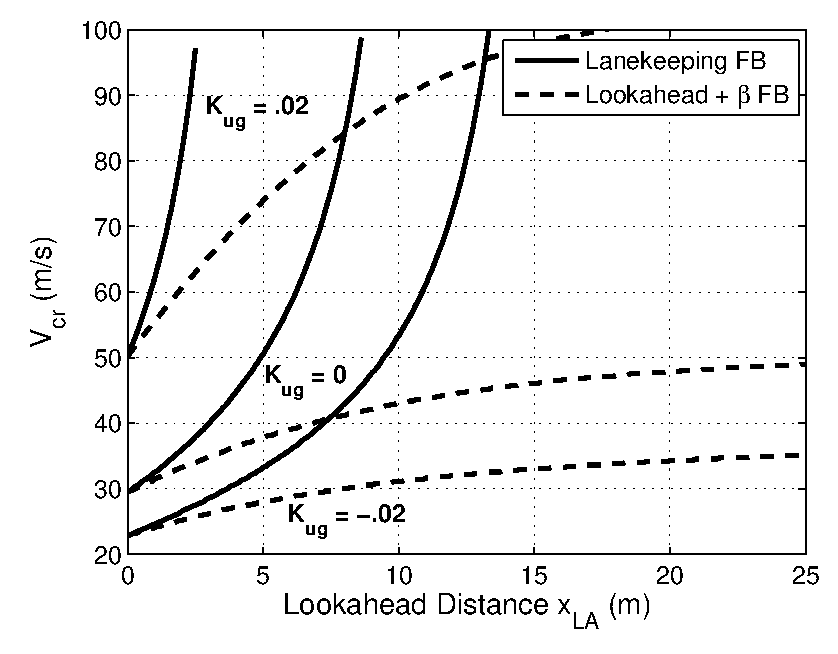
\includegraphics[width=\fullwidth]{VcrPlot.eps}
\caption[Maximum speed for closed-loop stability for the original lookahead feedback and the modified feedback with sideslip tracking.]{Maximum speed for closed-loop stability for the original lookahead feedback and the modified feedback with sideslip tracking. Results are based on
eigenvalue computations of the $A$ matrix of the linear vehicle model.}
\label{fig:VcrPlot}
\end{figure} 
Even in situations where the vehicle is in a 
neutral steer or oversteer configuration, the critical speed for closed-loop stability increases rapidly with lookahead distance. A different trend is present when
sideslip tracking is added to the steering feedback. Fig.~\ref{fig:VcrPlot} shows that the critical speeds for 
stability increase very slowly as a function of lookahead distance.

\section{Incorporating Sideslip Information Into \newline Steering Feedforward}
\label{sec:goodFFW}
 
 Given the trade-off between path tracking and stability when sideslip-path alignment is enforced via feedback, a promising approach
 is to replace vehicle sideslip  $\beta$ in (\ref{eqn:vveq}) with the predicted steady-state sideslip value $\beta_\mathrm{ss}$ 
 for a given vehicle speed and curvature. 

The rear tire slip for a fixed track vehicle, assuming small angles, is given by 
\begin{equation}
\alpha_\mathrm{r} = \beta - \frac{br}{U_x}
\end{equation} 
At steady-state, $\alpha_\mathrm{r}=\alpha_\mathrm{r}^\mathrm{FFW}$ from (\ref{eqn:steadyffw}) and $r=\kappa U_x$, yielding the following feedback control law:
\begin{subequations}
\begin{align}
\label{eqn:betass}
\delta_\mathrm{FB} &=-k_\mathrm{P} \left(e+x_\mathrm{LA} (\Delta\Psi+\beta_\mathrm{ss}) \right) \\
\beta_\mathrm{ss}  &= \alpha_\mathrm{r}^\mathrm{FFW} + b\kappa
\end{align}
\end{subequations}
The effect of this change is to remove the steering controller's dependence on \textit{real-time} sideslip information. The steering
controller will now act to align the vehicle's predicted \textit{steady-state} sideslip along the desired path. Since the controller no
longer has feedback on vehicle sideslip, the state matrix equation $A$ for the closed-loop system dynamics is now 
once again given by (\ref{eqn:Amatrix}b), which was shown to have desirable stability
properties as a function of $K_\mathrm{ug}$ and $x_\mathrm{LA}$ (Fig.~\ref{fig:VcrPlot}). The sideslip now affects the vehicle
path tracking dynamics through the feedforward path, since the predicted steady-state sideslip $\beta_{ss}$ depends only on the
desired speed $U_x$ and curvature $\kappa$ as well as the feedforward tire model. 

The $B$ matrix in (\ref{eqn:Amatrix}) now becomes: 

\begin{subequations}
\label{eqn:newB}
\begin{align}
	B &=\left[0 \hspace{2 mm} -U_x \hspace{3 mm} \frac{a C_\mathrm{f} (G_\mathrm{FFW}+G_\beta)}{I_\mathrm{z}} \hspace{3 mm}  \frac{C_\mathrm{f} (G_\mathrm{FFW}+G_\beta)}{mU_x}\right]^T \\
	G_\beta &= U_x^2\frac{ma}{L}\frac{k_\mathrm{p}x_\mathrm{LA}}{C_\mathrm{r}}
\end{align}
\end{subequations}

Assuming perfect knowledge of the feedforward tire model, the resulting steady-state lateral path deviation will be zero at all vehicle speeds,
as shown in Fig.~\ref{fig:linError2}.
\begin{figure}[h]
\centering
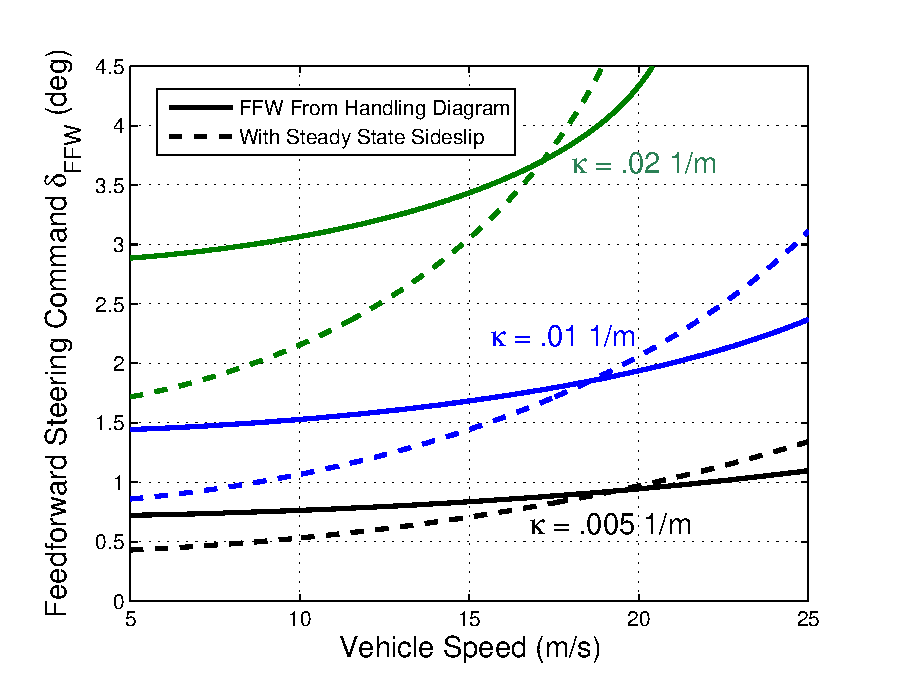
\includegraphics[width=\fullwidth]{FFWplot.eps}
\caption{Effect of incorporating sideslip behavior into feedforward steering command $\delta_\mathrm{FFW}$, as a function of 
vehicle speed and desired path curvature.}
\label{fig:ffwplot}
\end{figure}
However, error in the feedforward tire model will result in steady-state lateral path deviation.
The effect of incorporating steady-state sideslip into the feedforward control is shown in Fig.~\ref{fig:ffwplot}. The feedforward
steering command $\delta_\mathrm{FFW}$ as a function of path curvature and vehicle speed is plotted both for the original feedforward control law (\ref{eqn:Amatrix}c) as well as the sideslip-incorporating
feedforward command (\ref{eqn:newB}). 

\section{Experimental Results}
\label{sec:expresults}

\subsection{Experimental Setup}

Experimental data was collected on ``Shelley", an Audi TTS equipped 
with an electronic power steering motor for autonomous steering and active brake booster and throttle by wire for
longitudinal control (Fig.~\ref{fig:shelleyPicC2}). The testbed is also
equipped with an integrated Differential Global Positioning System (DGPS) and Inertial Measurement Unit (IMU) in order to obtain
 global vehicle states. Mentioned previously in \S \ref{sec:arv}, this is the same vehicle developed by
Stanford and Audi to autonomously drive the Utah Salt Flats and Pikes Peak Hill Climb \cite{saltflats}. 

\begin{figure}[h]
\centering
\includegraphics[width=\fullwidth]{experimentInfo.jpg}
\caption{Audi TTS used for experimental validation.}
\label{fig:shelleyPicC2}
\end{figure}

\begin{figure}[h]
\centering
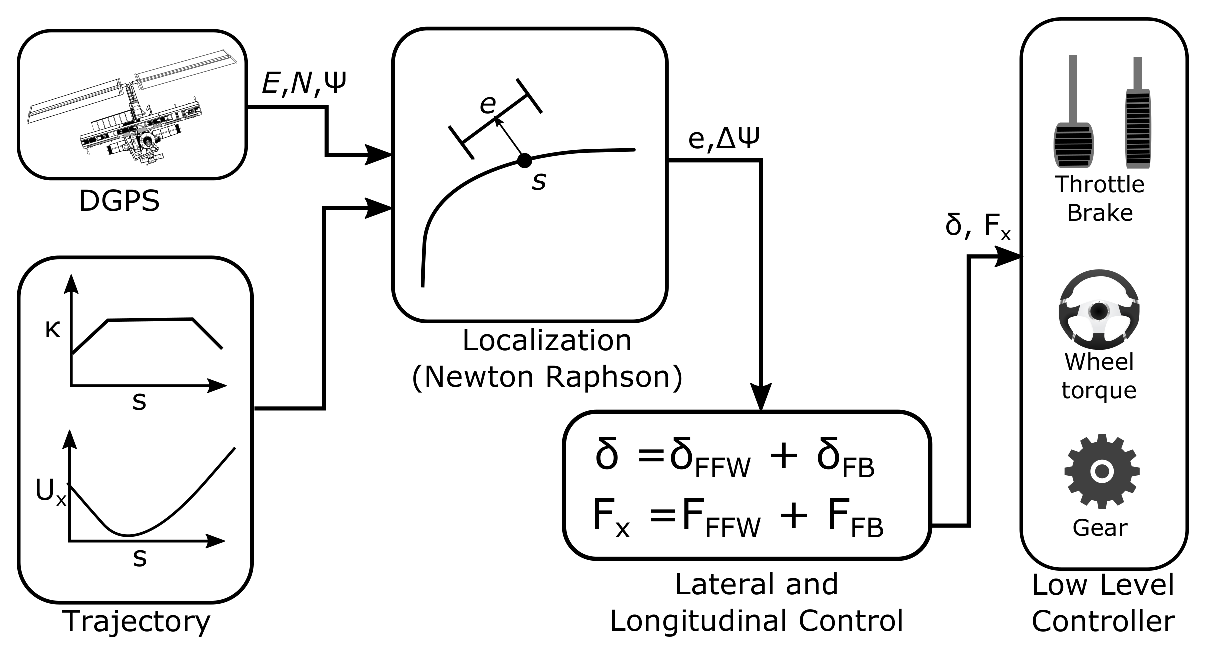
\includegraphics[width=.85\fullwidth]{expSetupC2.eps}
\caption{Diagram showing controller setup.}
\label{fig:expSetupC2}
\end{figure}
\newpage 
The overall controller setup is shown in Fig.~\ref{fig:expSetupC2}. At each time step,
the differential GPS unit obtains precise ( $<$ 2 cm) measurements of the vehicle
 global East and North coordinates as well as the vehicle angular orientation $\Psi$.
 The controller also has prior knowledge of the desired high level trajectory, 
 consisting of the clothoid curvature profile from Theodosis \cite{theodosis} and 
 the speed profile from Kritayakirana \cite{mickthesis}. 
Vehicle parameters for the Audi test vehicle and the lookahead feedback
 gains are presented in Table \ref{tb:params}.

 
 \begin{table}[h]
\begin{center}
\caption{Vehicle Parameters}\label{tb:params}
\begin{tabular}{lccc}
Parameter & Symbol & Value & Units \\\hline
Vehicle mass & $m$ & 1500 & kg \\
Yaw moment of inertia & $I_z$ & 2250 & $\mathrm{kg \cdot m}^2$\\
Front axle to CG & $a$ & 1.04 & m\\
Rear axle to CG & $b$ & 1.42 & m\\
Front cornering stiffness & $\mathrm{C}_\mathrm{f}$ & 160 & $\mathrm{kN \cdot rad}^{-1}$ \\
Rear cornering stiffness & $\mathrm{C}_\mathrm{r}$ & 180 & $\mathrm{kN \cdot rad}^{-1}$ \\
Lookahead Distance		 & $x_\mathrm{LA}$         & 14.2 & $\mathrm{m}$ \\
Lookahead Gain         & $k_\mathrm{p}$         & 0.053 & $\mathrm{rad/m}$ \\\hline
\end{tabular}
\end{center}
\end{table}
 \newpage
 The global East, North, and $\Psi$ measurements
are fed into a Newton-Raphson localization algorithm, which finds the closest point from the vehicle
center of gravity to the path and outputs values of $e$ and $\Delta\Psi$. The resulting steering
command is generated using the feedback-feedforward control laws developed in this chapter. 
In addition, to track the desired speed profile, a longitudinal force command is generated with a basic 
proportional control law presented by Kritayakirana \cite{mickthesis}. Finally, a low level
controller developed by Audi and Stanford maps the
steer angle and force command into the resulting throttle, brake, steering wheel torque, and gear shift commands.  
The control loop operates at 200 Hz, with computations performed on a dSPACE MicroAutobox real-time embedded computer. 

The site for data collection was a 3.1 mile paved racing circuit (friction coefficient $\mu \approx$ 1) at Thunderhill Raceway Park in Willows, CA.
Fig.~\ref{fig:thPic} shows an overhead plot of the race track as well as the desired racing line. The desired racing
line is parameterized as a curvature profile $\kappa(s)$ that varies with distance along the path. The curvature
profile associated with the racing line is shown in Fig.~\ref{fig:traj}
along with a typical longitudinal velocity profile $U_x$ from the path planner.

\begin{figure}[h]
\centering
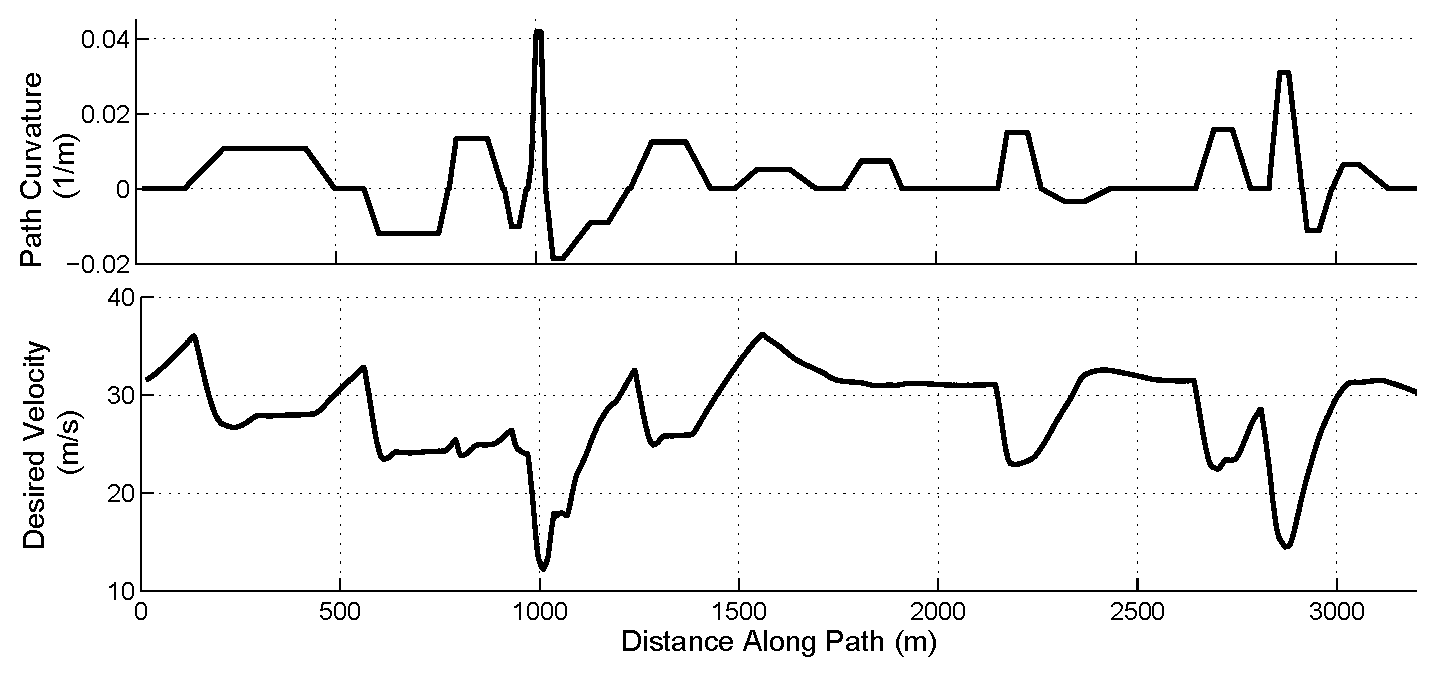
\includegraphics[width=\fullwidth]{traj.eps}
\caption{Curvature and velocity profile inputs for steering controller as a function of distance along racing line.}
\label{fig:traj}
\end{figure}


\begin{figure}[h]
\centering
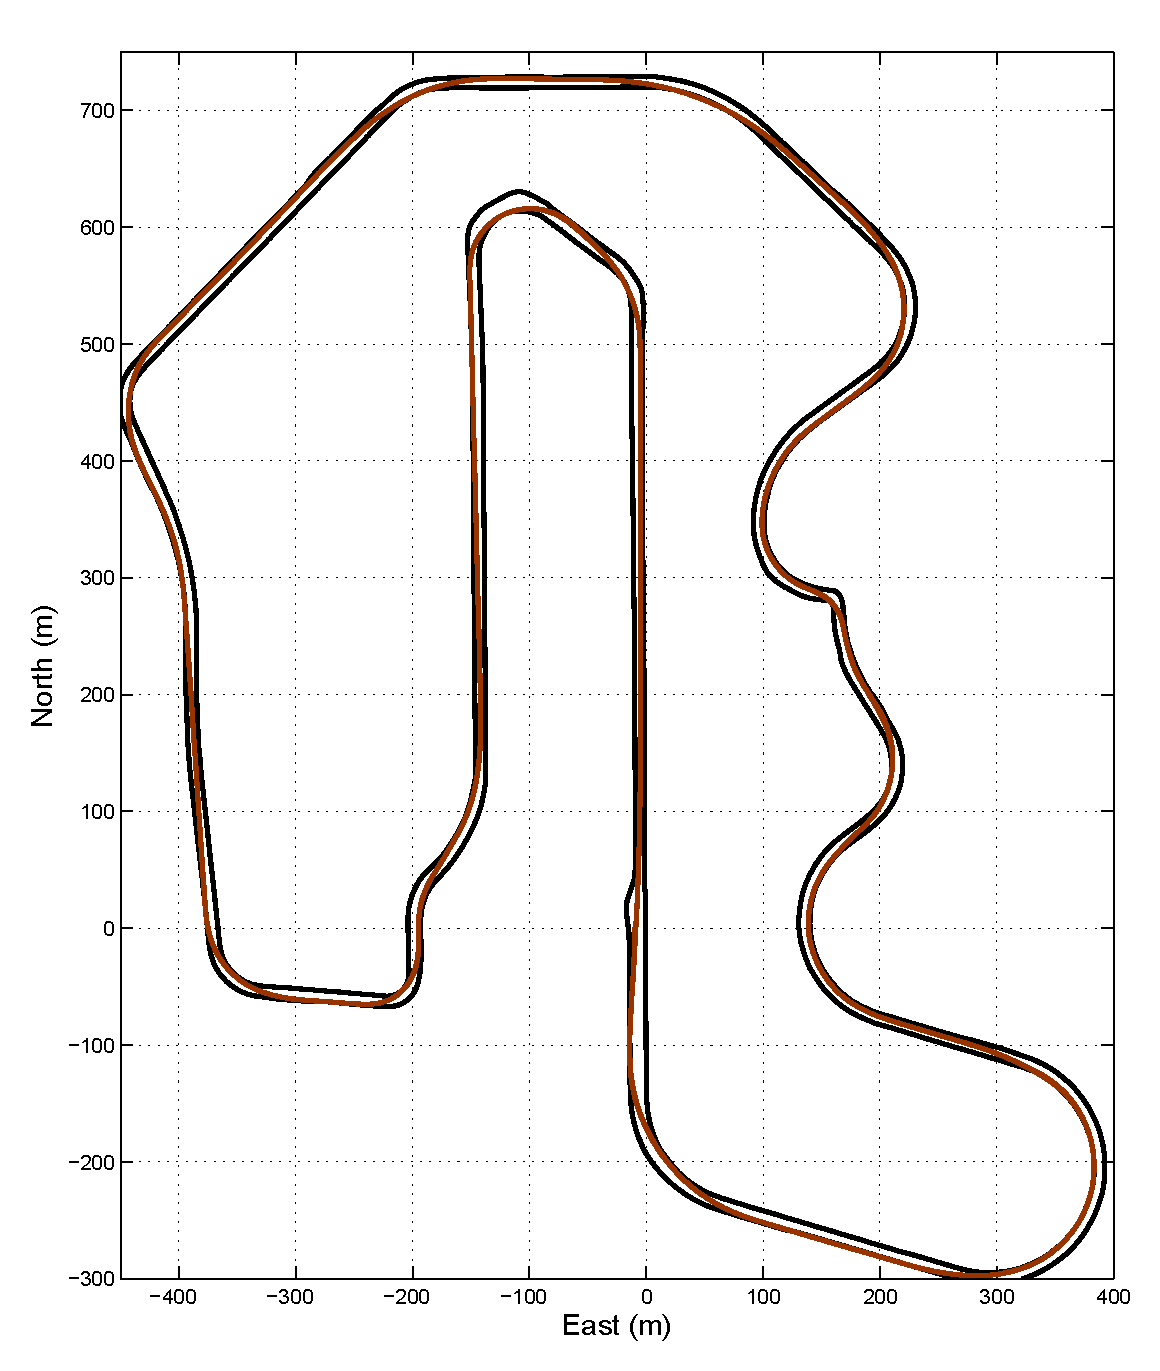
\includegraphics[width=\fullwidth]{racingLine.eps}
\caption{Desired path for steering controller to follow.}
\label{fig:thPic}
\end{figure}

\section{Experimental Testing of Sideslip Feedback \newline Controller}

The steering feedback controller with sideslip-path tangency presented in Section \ref{sec:betafb} offers very low path tracking error, but at the
expense of reduced stability margins. To test this controller safely at the limits of handling, experimental data was collected on a
constant radius turn in an open parking lot at two constant speeds. The results of this test are shown in Fig.~\ref{fig:wipeout}. As a baseline, the
feedback controller with sideslip (\ref{eqn:vveq}) from Section \ref{sec:betafb} is compared to the original lookahead feedback controller (\ref{eqn:lookahead}). 
The feedforward steering based on the nonlinear handling diagram (\ref{eqn:steadyffw}) is used in both cases. 
For the case where the speed is 10 m/s, the resulting steady-state acceleration is 7 $\mathrm{m/s^2}$, and both steering controllers maintain stability of the vehicle. 
In addition, incorporating sideslip-path tangency into the feedback control law results in significantly lower path tracking errors compared to the baseline
lookahead feedback controller.

 However, when the speed is increased to 13 m/s, the resulting steady-state lateral acceleration is 9 $\mathrm{m/s^2}$,
and the sideslip feedback controller becomes unstable, causing the vehicle to spin out spin, as demonstrated by the plots of yaw rate and sideslip. For the same conditions,
the baseline lookahead controller remains stable. The issue with the sideslip feedback controller is shown in the plot of vehicle sideslip and heading
error. As the vehicle heading error decreases and becomes unstable around $s = $ 170 m, the feedback controller does not intervene because the
 vehicle's velocity vector remains tangent to the path (i.e. $\Delta\Psi + \beta =$ 0). A counter steering action is finally provided at $s = $ 190 m, but at this point the vehicle
has already spun out.

\begin{figure}
\centering
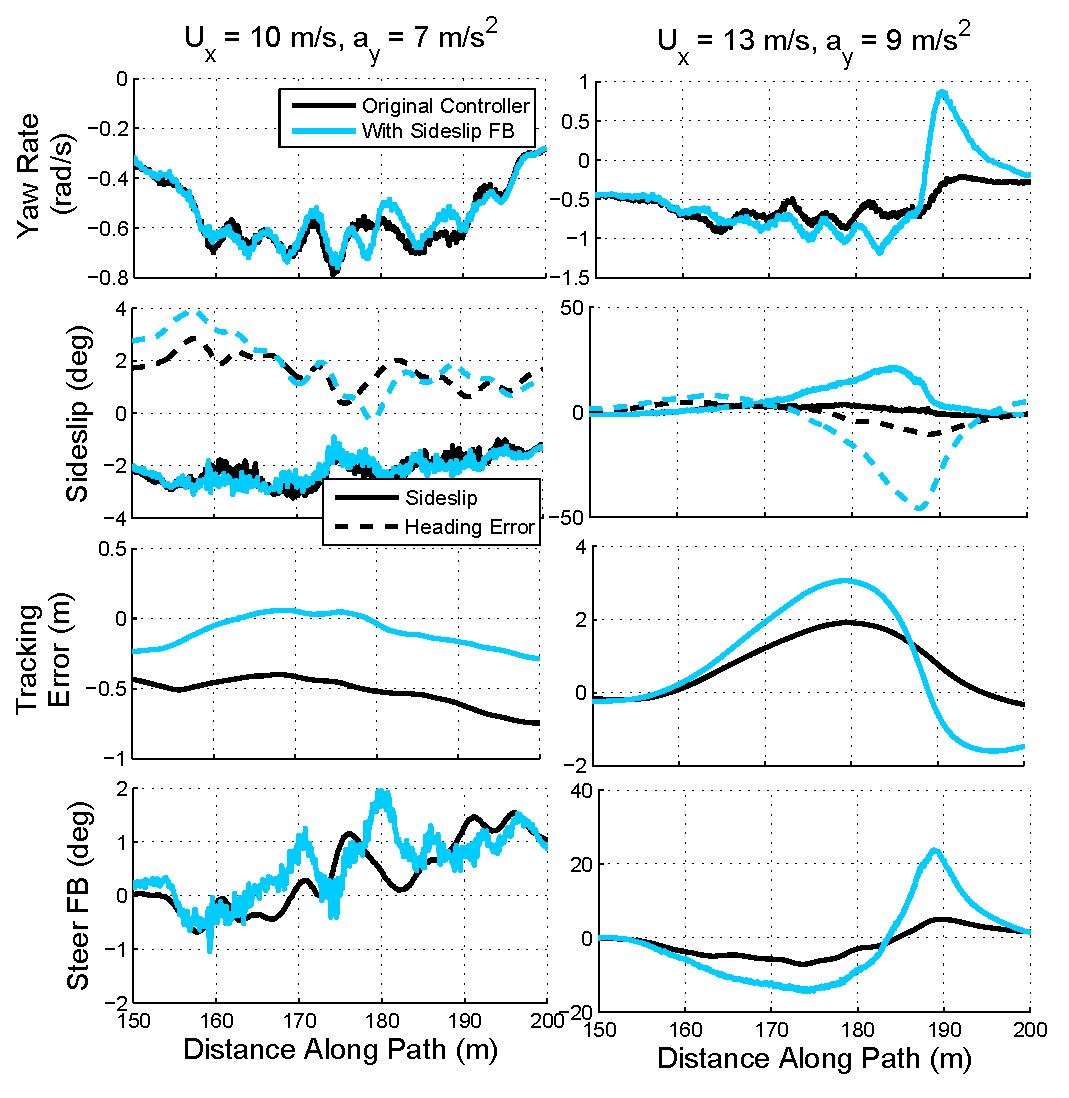
\includegraphics[width=\fullwidth]{wipeout.eps}
\caption[Parking lot test for constant radius turning at 10 m/s and 13 m/s.]{Parking lot test for constant radius turning at 10 m/s and 13 m/s. Resulting steady-state accelerations are 7 $\mathrm{m/s^2}$ and 9
$\mathrm{m/s^2}$. Steering feedback with sideslip is compared to original lookahead steering controller.}
\label{fig:wipeout}
\end{figure}


\section{Experimental Data from Racetrack}

Fig.~\ref{fig:betaComparison} shows experimental data taken over a 3 km subset of the entire racetrack,
excluding portions of the course where there is little vehicle cornering. The experimental data is plotted for two separate steering
controllers. The first controller is the baseline controller described in \S \ref{sec:controllerC2}, with the
steering feedback provided by the lookahead system and the feedforward steering given by the steady-state handling diagram. The second controller uses the same lookahead feedback, but incorporates the steady-state sideslip
behavior into the feedforward steering to align the vehicle's velocity vector with the path heading (\S \ref{sec:goodFFW}).
Note that the controller where real-time sideslip was incorporated into the steering feedback (\S \ref{sec:betafb}) was not tested, as there is a high likelihood
of vehicle instability near the limits of handling given the results from the previous parking lot test. The same longitudinal controller is used for both cases in order to
 brake into the entry of turns and accelerate out of turn exits. For this lap, the peak longitudinal deceleration is -8 $\mathrm{m/s^2}$ and
 peak lateral acceleration is 8 $\mathrm{m/s^2}$.
 
\begin{figure}[h!]
\centering
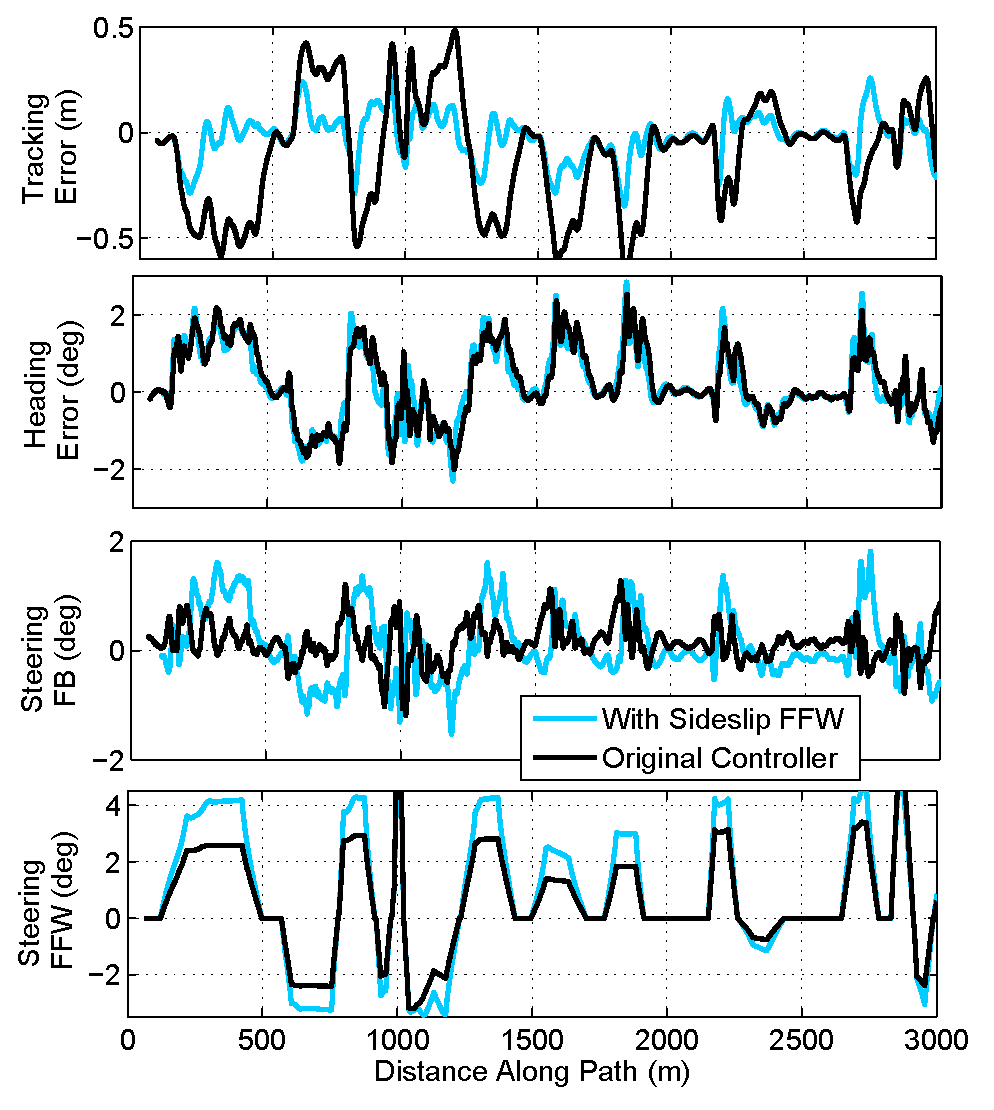
\includegraphics[width=\fullwidth]{betaCompensation.eps}
\caption{Experimental data with combined acceleration magnitude 8 $\mathrm{m/s^2}$ over a 3 km stretch of Thunderhill Raceway Park. Results are
shown for both the baseline FB-FFW controller and the modified controller with sideslip tracking in the feedforward loop.}
\label{fig:betaComparison}
\end{figure}

The results in Fig.~\ref{fig:betaComparison} show that lateral path deviation $e$ is reduced when incorporating 
steady-state sideslip in the feedforward control law. This confirms the expected results from the analysis performed in \S \ref{sec:predSS}
and \S \ref{sec:goodFFW}. Note that while the lateral path deviation is smaller, the levels of vehicle heading error $\Delta\Psi$ remain roughly the
same. This matches the predicted result in Fig.~\ref{fig:linError2}. The steering controller will align the vehicle's
velocity vector with the path, not the vehicle's heading, and due to a vehicle's tendency to develop a steady-state sideslip angle,
 a non-zero heading error $\Delta\Psi$ is in general necessary for zero steady-state lateral path deviation,
 as shown by the schematic in Fig.~\ref{fig:SSerror}.

 For a better comparison of the lateral path deviation, Fig.~\ref{fig:errhist} shows histograms of the lateral tracking
error $e$ for both controllers at three levels of peak lateral acceleration. The baseline controller keeps the vehicle within 0.5 meters
 on either side of the desired path, with a large
amount of variation in the resulting histogram. An interesting observation is that the 
histogram is not symmetric. In general, the raceway has more left turns than right turns, and as Fig.~\ref{fig:linError} indicates, at
high speeds the baseline controller will track toward the outside of the turn. This tendency is manifested experimentally in the asymmetric nature
of the histograms. The histograms for the improved controller show a much tighter distribution on the lateral path tracking 
error. The path tracking error generally remains within 10-15 cm on either side of the lane boundary and contains less of a bias towards tracking
on the outside of turns.  
 
\begin{figure}
\centering
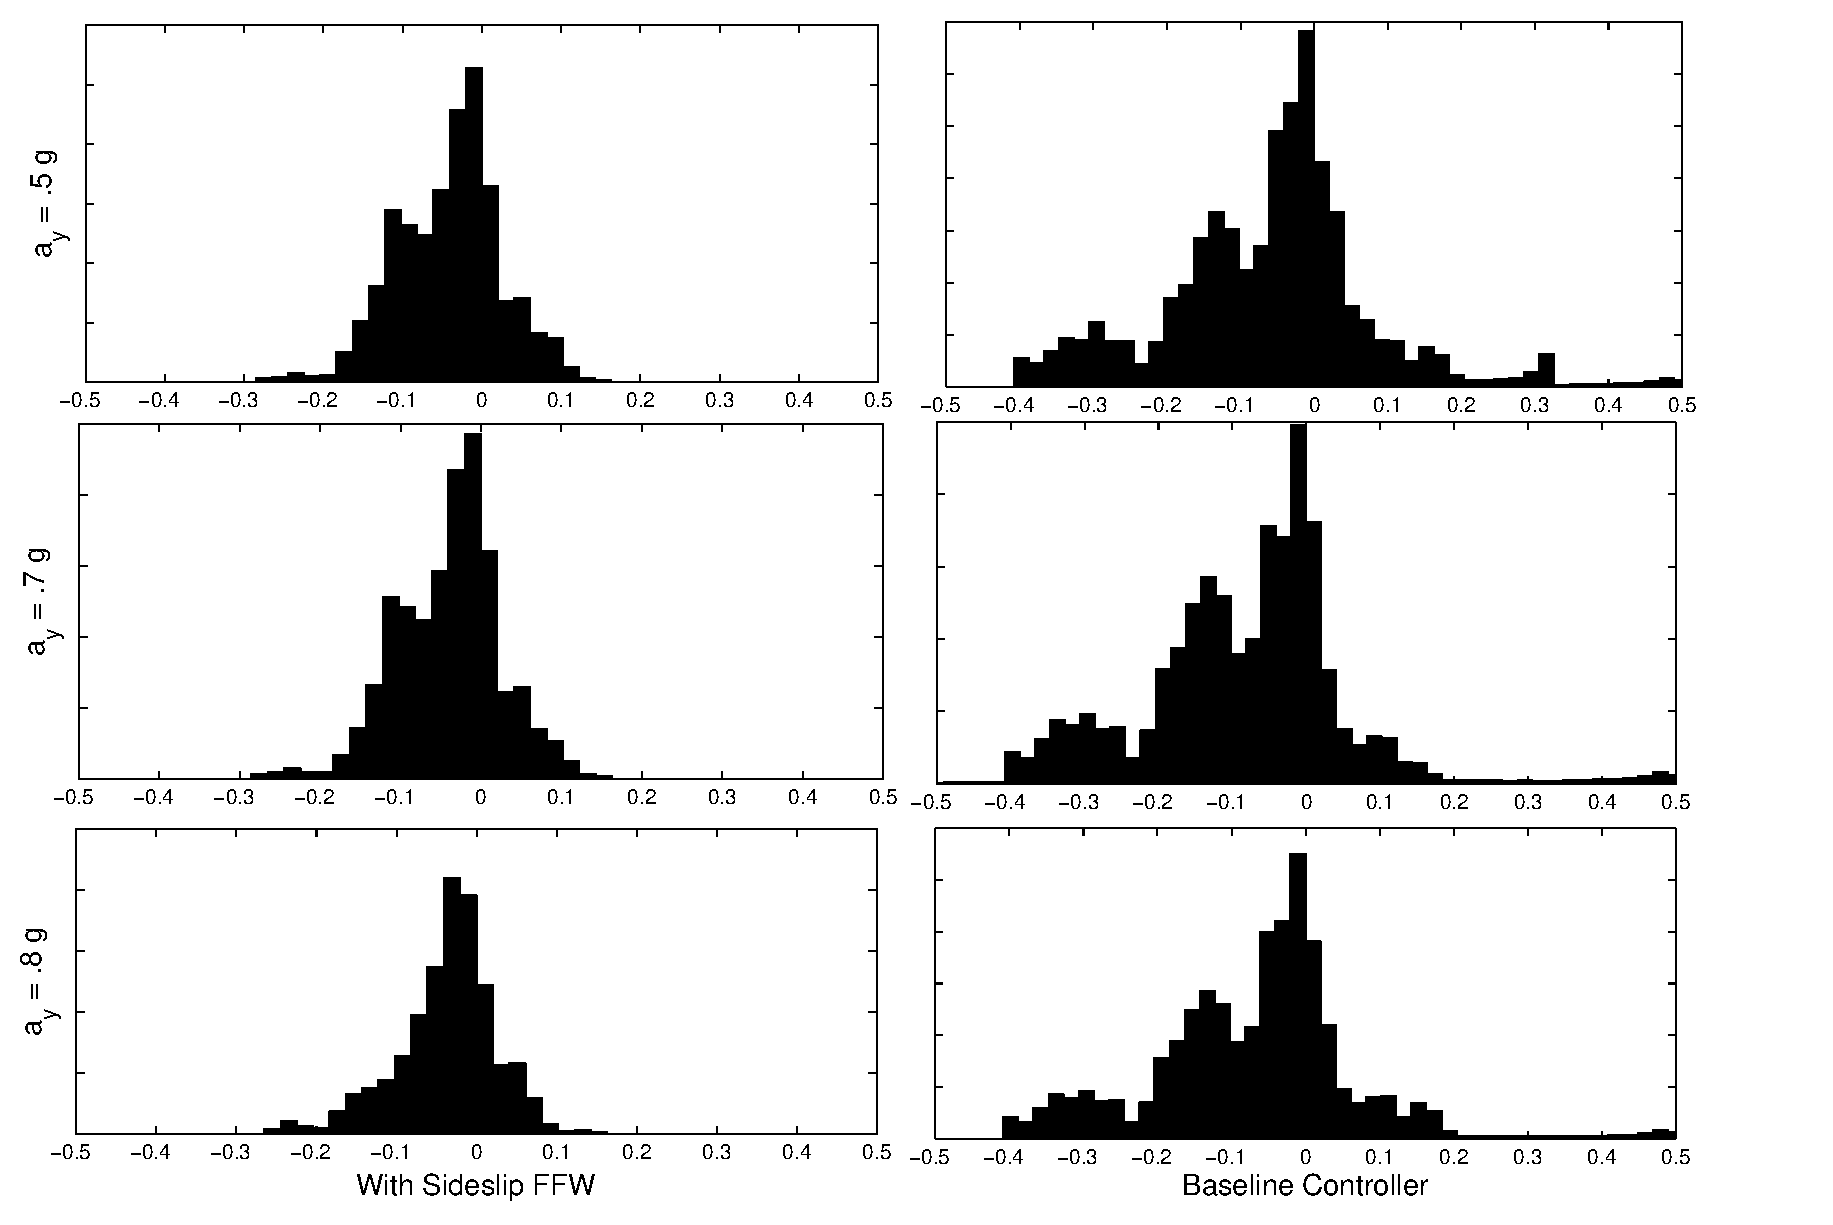
\includegraphics[width=\fullwidth]{errhist.eps}
\caption[Histogram of path tracking error for six laps around the track.]{Histogram of path tracking error for six laps around the track. Left column represents performance of controller
with feedforward sideslip tracking, and right column is baseline controller with feedforward from
the steady-state handling diagram. Path tracking error is in meters.}
\label{fig:errhist}
\end{figure}

As the lateral acceleration increases beyond 0.8 g and the vehicle approaches the handling limits, the steering controller
remains stable and well-damped, although the tracking performance begins to degrade. Fig.~\ref{fig:atTheLimits} shows experimental
data for a lap around Thunderhill Raceway park with peak lateral and longitudinal accelerations of 0.95 g. At several points along the
track, the tracking error increases above 0.5 m, significantly higher than the levels of path deviation seen at 0.8 g of vehicle acceleration.
The reasons for this are three-fold. 

\begin{figure}
\centering
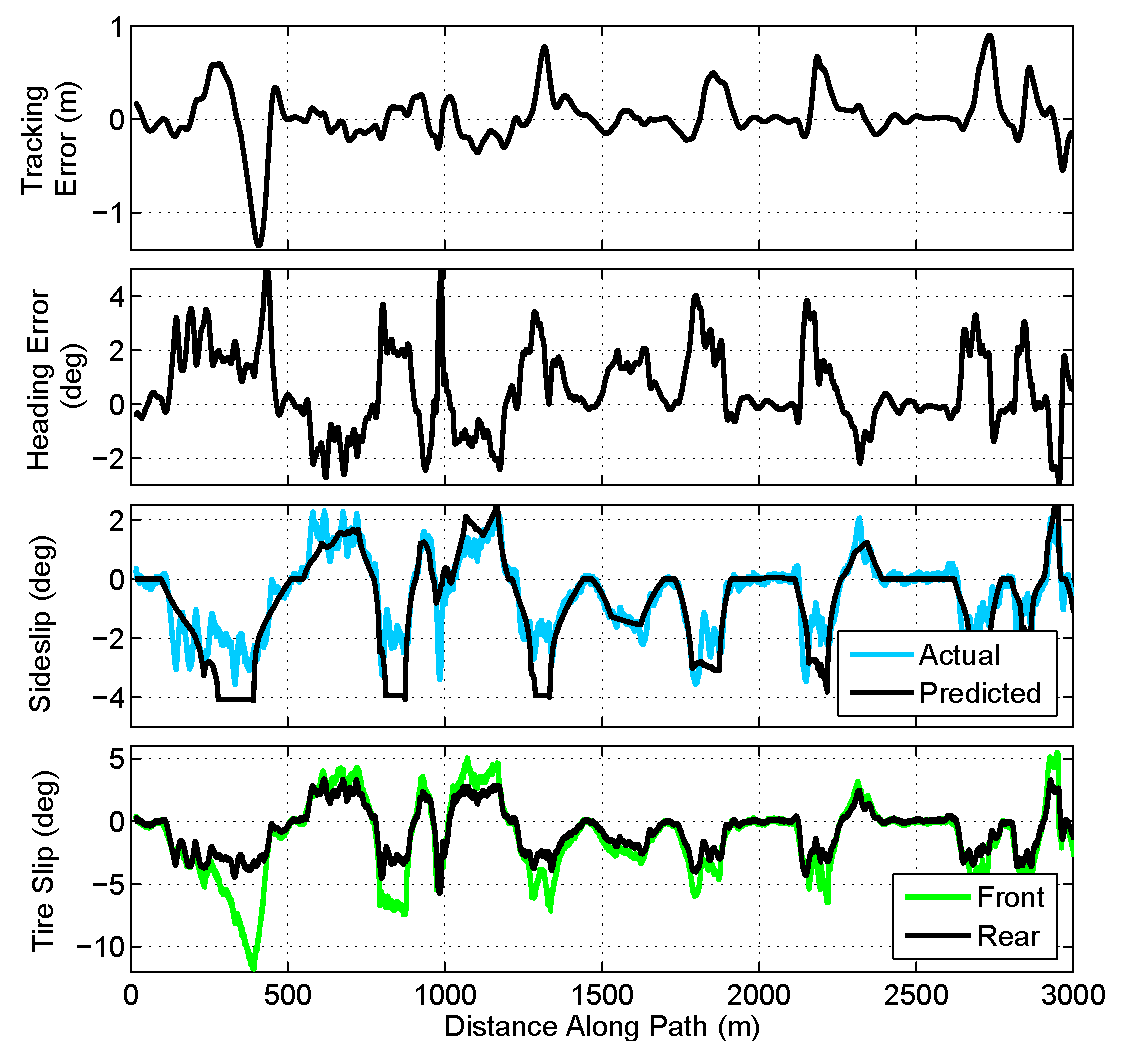
\includegraphics[width=\fullwidth]{atTheLimits.eps}
\caption{Experimental data with combined acceleration magnitude 9.5 $\mathrm{m/s^2}$ over a 3 km stretch of Thunderhill Raceway Park.}
\label{fig:atTheLimits}
\end{figure}

First, the sharp drop in front tire slip from $s$ = 300 to 400 meters indicates that the 
 lateral force demand for the front tires has exceeded the available friction at that region of the track. As a result, the vehicle
 understeers heavily and tracks well to the outside of the left-hand turn, resulting in a large negative tracking error.
At this point, there is nothing the steering controller can do to bring the vehicle back to the desired path, and the vehicle must alter its
desired trajectory to become less aggressive, either by slowing down or reducing the turn curvature. Second, the steady-state feedforward controller requires an accurate estimate of the vehicle parameters in order to estimate
the steady-state sideslip in (\ref{eqn:betass}). From $s$ = 700-800, 1300-1400, 1800-1900, and 2200-2300 meters along the track, there are observable
discrepancies between the predicted feedforward sideslip and the actual vehicle sideslip, as measured by the GPS-INS. This plant-model mismatch results in significant path tracking errors at those portions of the racing circuit. Finally, the feedforward
model in (\ref{eqn:betass}) assumes steady-state conditions. As the vehicle approaches the limits of handling, transient vehicle
dynamics can result in larger path deviations as well.

The lap-to-lap learning algorithms presented in Chapter 4 focus on reducing the latter two sources of
 error by gradually learning a better feedforward model of the
vehicle dynamics over time. For situations where a vehicle repeats a 
given trajectory multiple times, iterative learning control (ILC)
is a promising technique for refining the feedforward input to improve
 the reference tracking performance of the controller. Additionally, online estimation
approaches can also be used to gradually improve knowledge 
of difficult-to-measure parameters such as friction and vehicle cornering
stiffness.

% %=======================================================================
\section{Conclusion}

This chapter describes the design of a feedback-feedforward controller capable of path tracking at the limits of handling. Desirable
 path tracking behavior occurs when the vehicle sideslip is aligned
with the desired path heading. However, directly incorporating this behavior into a feedback steering control law results in 
a closed-loop controller with poor stability margins. 
A better approach for combined path tracking and stability is to align the steady-state vehicle sideslip 
with the desired path heading through the feedforward steering command. 

The benefit of the presented work is a controller design that provides low path tracking error over a large
range of vehicle lateral accelerations. More importantly, the lateral path tracking improvement is achieved without
sacrificing the robust stability properties of the lookahead steering feedback. Results from
a histogram analysis quantitatively indicate that the improved feedforward command reduces lateral path deviation from the baseline
controller by more than fifty percent. One potential drawback is that this feedforward approach is sensitive to vehicle model uncertainty, especially at the physical
limits of handling where transient dynamics become prevalent. Chapter 4 will present iterative learning control
algorithms to improve the feedforward vehicle model and eliminate undesirable transient dynamics. 

 \textit{Note: This chapter reuses material previously published by the author in \cite{kapania}.}
% \begin{enumerate}
% \item \textit{Kapania and Gerdes. Design of a feedback-feedforward steering controller for accurate path tracking and stability at the limits of handling. Vehicle System Dynamics 2015 \cite{kapaniaVSD}} 
% \item \textit{Kapania and Gerdes. An Autonomous Lanekeeping System for Vehicle Path Tracking and Stability at the Limits of Handling. AVEC 2014 \cite{kapania}.}
% \end{enumerate}

%\\